% This is samplepaper.tex, a sample chapter demonstrating the
% LLNCS macro package for Springer Computer Science proceedings;
% Version 2.20 of 2017/10/04
%
\documentclass[runningheads]{llncs}
%
\usepackage{graphicx}
\usepackage{float}
\usepackage{subcaption}
\captionsetup{compatibility=false}

% Used for displaying a sample figure. If possible, figure files should
% be included in EPS format.
%
% If you use the hyperref package, please uncomment the following line
% to display URLs in blue roman font according to Springer's eBook style:
% \renewcommand\UrlFont{\color{blue}\rmfamily}

\begin{document}
%
\title{Bachelor Dissertation}
%
%\titlerunning{Abbreviated paper title}
% If the paper title is too long for the running head, you can set
% an abbreviated paper title here
%
\author{Kasper Engelen\and
		Jonathan Meyer\and
		Dawid Miroyan\and
		Igor Schittekat}
%
%
\institute{University of Antwerp}
%
\maketitle              % typeset the header of the contribution
%
\begin{abstract}
This document reports our findings regarding the final dissertation. The sections and subsections correspond to the assignments given to us. In this project we worked with a simulator called Stride, developed at the University of Antwerp. We explore various concepts within computational epidemiology through the use of this program. 

\keywords{Computational Epidemiology  \and Dissertation}
\end{abstract}
%
%
%
\section{Simulation}
\subsection{Stochastic Variation}
The first topic we consider is stochastic variation. Since the simulation uses a pseudo-random number generator, it's useful to inspect the influence of this stochasticity on the results of the simulation. Using the Stan tool which is provided with Stride, we collected data on 100 simulations with an identical configuration file. The only difference between executions is the RNG seed. When plotting the results, it becomes apparent that the amount of new cases per day follows a normal distribution. For the data we collected, we calculated a  mean of 33.33 new cases per day, and a variance of 1196.99. Looking at the plot for the cumulative cases per day, two 'categories' can be distinguished:  'outbreak' scenarios and 'extinction' scenarios. These cases are quite evenly spread, which explains the high variance for new cases per day. In the former, the curve has a sigmoid shape, indicating that the disease succesfully spread among the population. The latter scenario corresponds to the curves that are almost constant and are bounded by a value well under the population size. In these cases, the disease did not manage to spread, resulting in only a few infected people at the end of the simulation. This is likely explained by the initial infectation: if the first person to be infected is sufficiently isolated (either socially or by being surrounded by people who are immune), the disease doesn't have a chance to spread.\\
Figure \ref{casesPlots} shows the different scenarios. In the cumulative cases plot the 'extinction' senario is clearly visible at the bottom. The plot for new cases per day is very jagged, which can also be explained by the stochastic nature of the simulation.

\begin{figure}[h!]
	\centering
	\begin{subfigure}[b]{0.7\linewidth}
		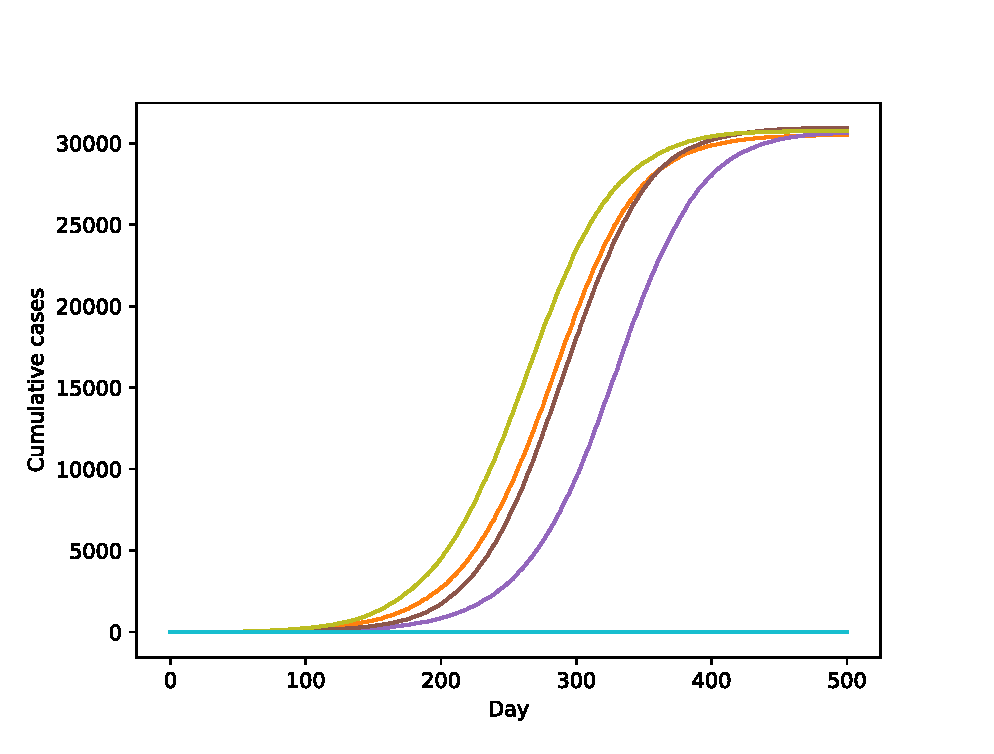
\includegraphics[width=\linewidth]{cases_cum.eps}
		\caption{Cumulative cases per day.}
	\end{subfigure}
	\begin{subfigure}[b]{0.7\linewidth}
		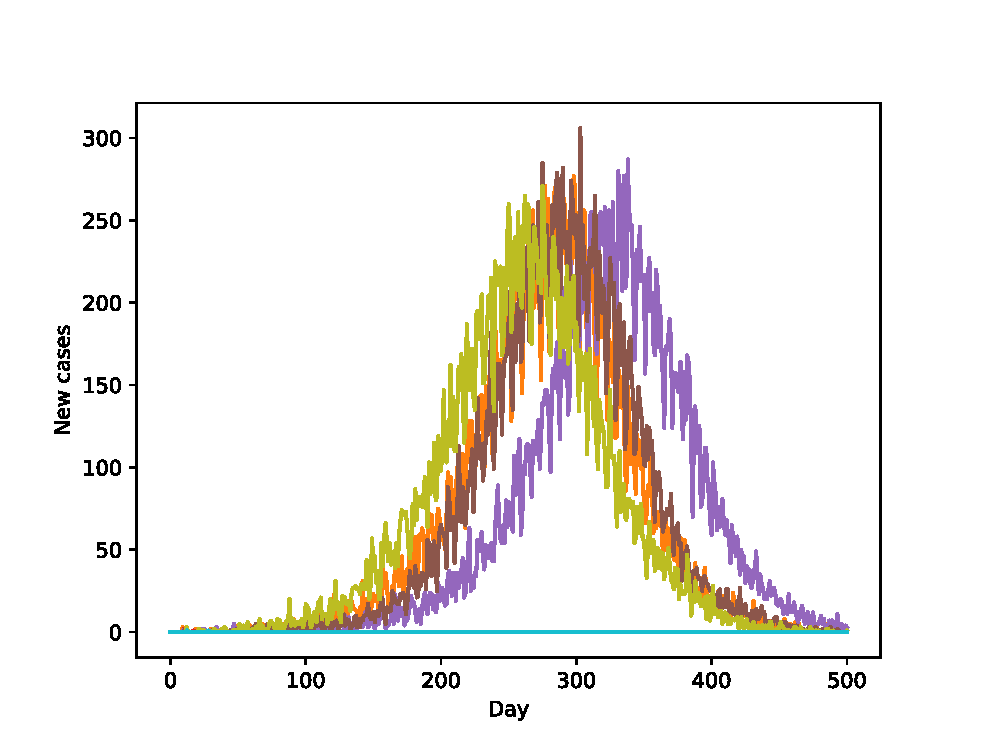
\includegraphics[width=\linewidth]{cases_per_day.eps}
		\caption{New cases per day.}
	\end{subfigure}
	\caption{Plots using different seeds}
	\label{casesPlots}
\end{figure}


\subsection{Extinction Threshold}
As discussed previously, it might be the case that only very few people become infected over the course of a simulation. This is referred to as extinction. There is a clear distinction between outbreaks and extinctions, so in this subsection we attempt to find an \emph{extinction threshold}.

\paragraph{}
Figure \ref{ETHist} gives the frequencies of the amount of infected people at the end of the simulations. The distinction between outbreaks and extinctions is quite clear from this histogram. There is one peak on the lower end of the x-axis, and there is a cluster on the higher-end.

\begin{figure}[!h]
	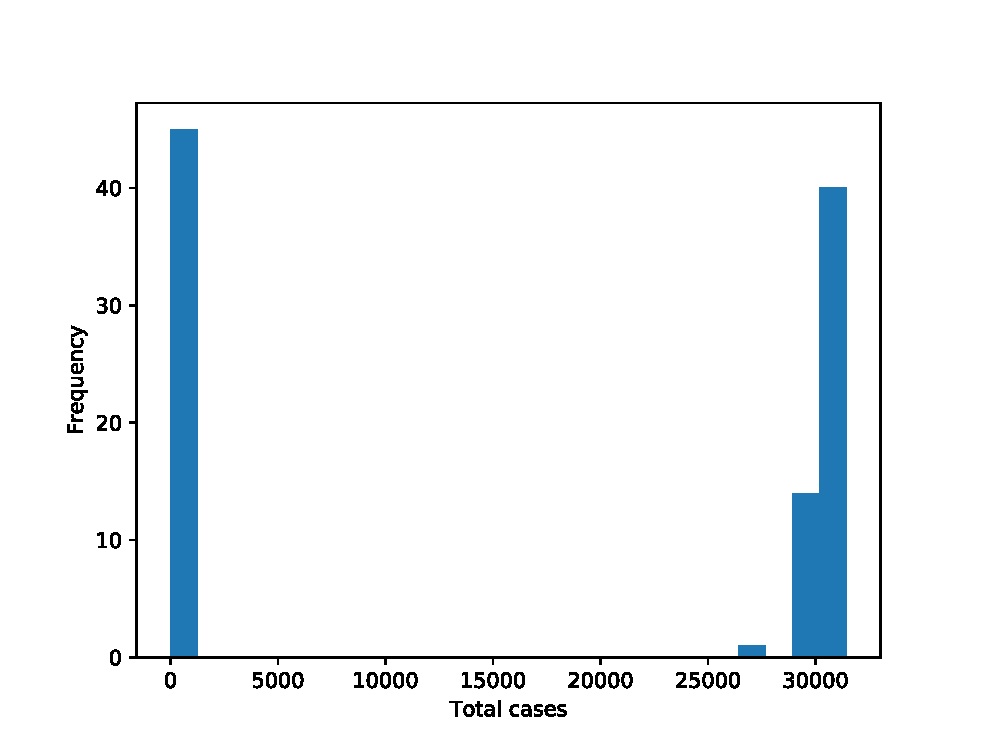
\includegraphics[width=\textwidth]{Hist.eps}
	\caption{Histogram showing the total amount of cases.} 
	\label{ETHist}
\end{figure}

\subsection{Immunity Level}
In order to make assumptions about the population's immunity level, we look at the simulated results for different values. Upon experimentation, it becomes apparent the immunity level is approximately 70\% of the population. Figure \ref{immLvlPlot} shows the average new cases per day for different immunity levels. The reference curve is also included. This plot was generated by taking the average of new cases per day over 20 simulations per immunity level. Using PyStride to simulate outbreaks, we narrowed down the immunity level $I$ to \( 0.705 \leq I \leq 0.7175 \).

\begin{figure}[H]
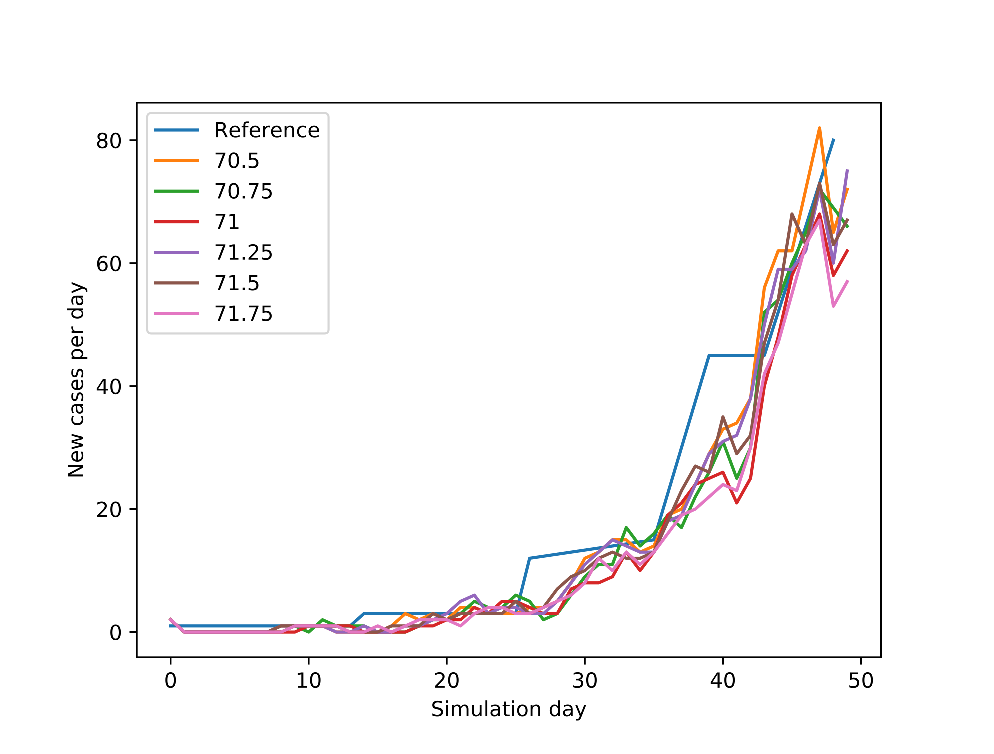
\includegraphics[width=\textwidth]{ImmLvl.eps}
\caption{New cases per day for different immunity levels.} 
\label{immLvlPlot}
\end{figure}


\subsection{Estimating $R_{0}$}
Now that we have a relatively decent estimate for the immunity level of the population, we can do an analogous exercise to estimate $R_0$. For this data, we fixed the immunity level to 70.5\%. Figure \ref{R0EstPlot} (a) shows the plot for each possible $R_0$ in the range $[12, 18]$ (average over 20 simulations). It's clear that the best candidates are 14, 15 or potentially 16. When we plot a more detailed plot for just those valued (average over 30 different simulations), it seems 15 is the best estimate for $R_0$.

\begin{figure}[h!]
	\centering
	\begin{subfigure}[b]{0.7\linewidth}
		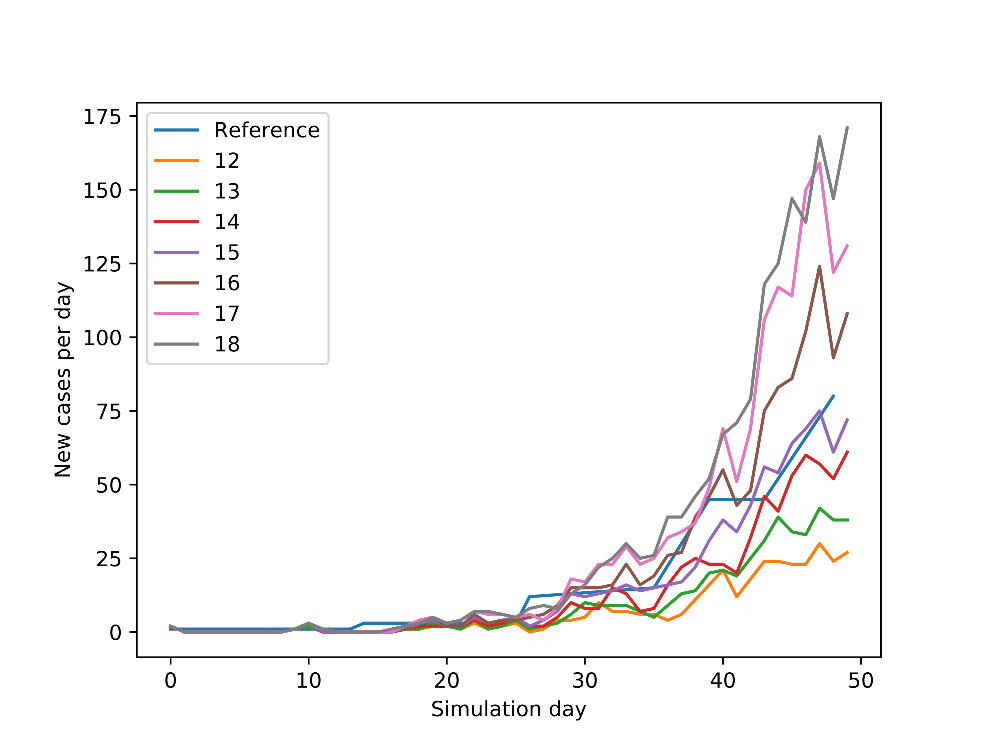
\includegraphics[width=\textwidth]{R0_all_20runs.eps}
		\caption{Overview of all potential $R_0$'s.} 	
	\end{subfigure}
	\begin{subfigure}[b]{0.7\linewidth}
		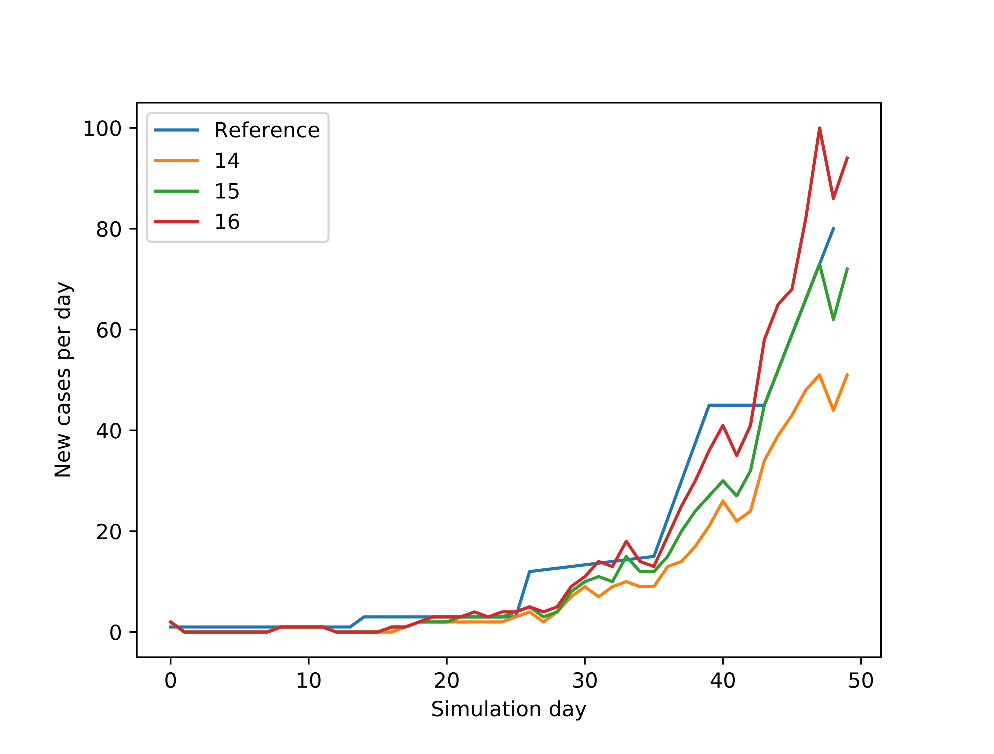
\includegraphics[width=\textwidth]{R0_detail_30runs.eps}
		\caption{More detailed look at $R_0$ candidates.} 
	\end{subfigure}
	\label{R0EstPlot}
	\caption{Plots for various values for $R_0$}
\end{figure}

\section{Population generation}

\subsection{Influence of demography}

\subsection{Vaccinating on campus}
By vaccinating the students, quickly after infected individuals appear in the population, we want to test whether so called 'catch-up' campaigns have a noticeable impact on an outbreak. \\
For these simulations, we generated a population where 60\% of people between the age of 18 and 26 attend high education. We then simulate scenarios where all students are either vaccinated on day 7 or not vaccinated at all. When looking at figure \ref{VaccinePlot}, the amount of new cases is the same in both scenarios on day 5 and 6. As the students are not vaccinated in both scenarios, some of them become infected and can spread the disease. Starting from day 7, where in one of the scenarios the susceptible students are vaccinated, the amount of new cases is lower than when not vaccinating.

\begin{figure}[h!]
	\centering
	\begin{subfigure}[b]{0.7\linewidth}
		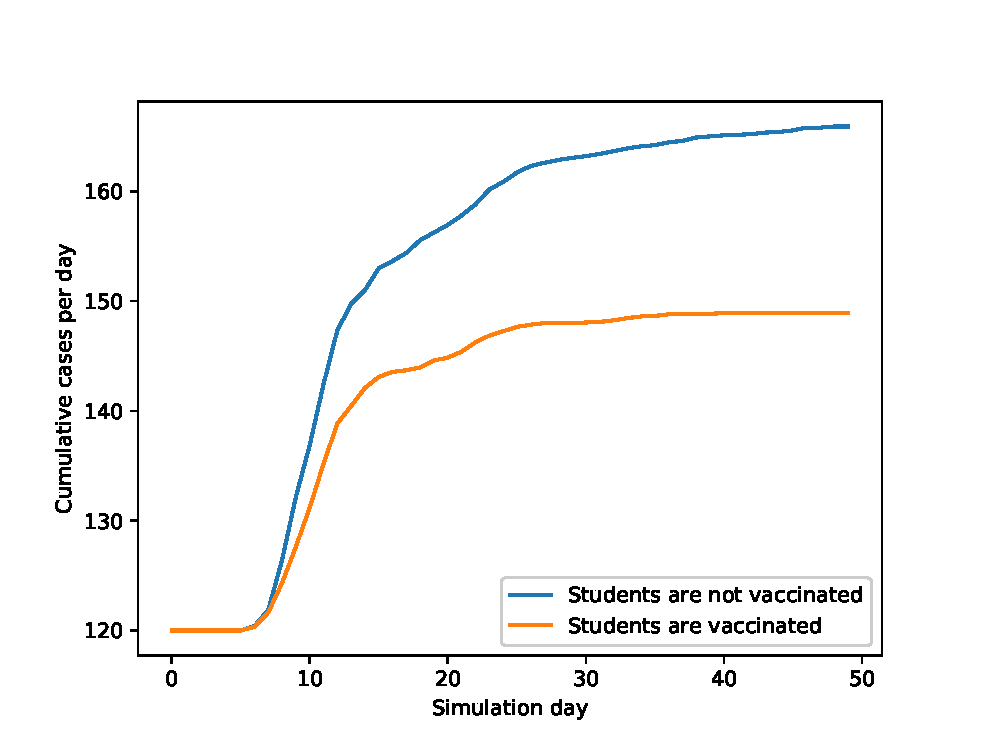
\includegraphics[width=\textwidth]{vaccinating_cases_cum_20runs.eps}
		\caption{Cumulative cases per day} 
	\end{subfigure}
	\begin{subfigure}[b]{0.7\linewidth}
		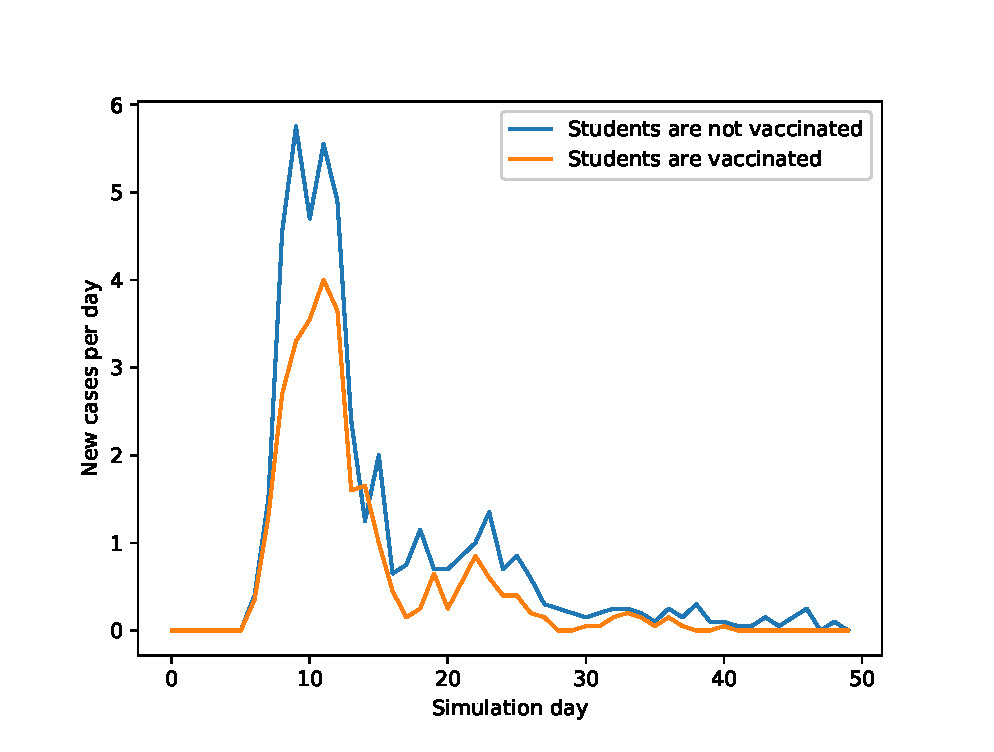
\includegraphics[width=\textwidth]{vaccinating_cases_per_day_20runs.eps}
		\caption{New cases per day.} 
	\end{subfigure}
	\label{VaccinePlot}
	\caption{Plots showing the impact of vaccinating students}
\end{figure}

\subsection{Commuting to work}
Another factor that is interesting to examine is the impact of commuting on disease spread. 

\end{document}
